\section{Results}
\label{sec:results}

In total, 3976 strides were extracted from the data of all horses. The performance results of the machine learning algorithms are presented in Table \ref{tab:ml_comparison_prepost}. As indicated in the table, the \gls{svm} model outperforms the four other algorithms in all of the subsets. Therefore, for the remainder of this chapter, we focus solely on reporting the results obtained from the \gls{svm} algorithm. The most significant features per subset and classification models performances, and the number of strides per subset are presented in Table \ref{featuresss results} and Table \ref{n_strides}, respectively.

\begin{table}[!htbp] 
    \centering
      \caption{Effect of different machine learning methods on the performance of the models, reported as mean ± standard deviation}% Add 'table' caption

    
    \resizebox{\linewidth}{!}{% 
\begin{tabular}{lccccccccc}
    
  \toprule
    
 & \multicolumn{9}{c}{Datasets and subsets}\\
\cmidrule(lr){2-10}

     & \multicolumn{3}{c}{Dataset 1} &  \multicolumn{3}{c}{Dataset 2} &  \multicolumn{3}{c}{Dataset 3}\\ [-1\medskipamount]
     & \multicolumn{3}{c}{(High/low intensity SET)} &  \multicolumn{3}{c}{(High intensity SET)} &  \multicolumn{3}{c}{(Low intensity SET)}\\
    \cmidrule(lr){2-4} \cmidrule(lr){5-7} \cmidrule(lr){8-10}
\multicolumn{1}{l}{Method}     & Walk & Trot & Walk+Trot & Walk & Trot & Walk+Trot & Walk & Trot & Walk+Trot\\
     \hline 
     \\\\[-5\medskipamount]
\gls{svm} & 95±2\% & 83±1\% & 82±2\% & 95±2\% & 86±4\% & 80±2\% & 100±0\% & 88±2\% & 83±3\%\\ [0.6 em]
\gls{knn} & 72±5\% & 71±6\% & 78±4\% & 82±5\% & 70±6\% & 57±8\% & 80±3\% & 73±5\% & 73±4\%\\ [0.6 em]
Decision tree & 77±4\% & 73±4\% & 81±3\% & 86±2\% & 69±8\% & 71±7\% & 90±2\% & 67±9\% & 75±5\%\\ [0.6 em]
Naive Bayes & 82±3\% & 70±7\% & 79±4\% & 86±2\% & 78±4\% & 72±7\% & 90±2\% & 70±6\% & 68±8\%\\ [0.6 em]
Logistic regression & 88±3\% & 78±6\% & 81±2\% & 88±2\% & 78±4\% & 78±5\% & 100±0\% & 70±5\% & 73±4\%\\ [0.1 em]

 \bottomrule



    \end{tabular}}
\label{tab:ml_comparison_prepost}
\end{table}

 \begin{sidewaystable}[!htbp] 
    \centering
      \caption{Features (mean and variability) with highest weight value based on different subsets, the best performing variability and the average performance results of the classification models from leave-one-subject-out cross validation (reported as mean ± standard deviation)}% Add 'table' caption

    
    \resizebox{\linewidth}{!}{% 
    \begin{tabular}{p{4.5cm}p{1cm}p{1cm}p{1cm}p{1cm}p{1cm}p{1cm}p{1cm}p{1cm}p{1cm}}
    
    \toprule
    

    \multicolumn{1}{l}{\bf Feature name} & \multicolumn{3}{c}{\bf Dataset 1 (High/low intensity SET)} &  \multicolumn{3}{c}{\bf Dataset 2 (High intensity SET)} &  \multicolumn{3}{c}{\bf Dataset 3 (Low intensity SET)}\\
    \cmidrule(lr){2-4} \cmidrule(lr){5-7} \cmidrule(lr){8-10}
     & \bf Walk & \bf Trot & \bf Walk+Trot & \bf Walk & \bf Trot & \bf Walk+Trot & \bf Walk & \bf Trot & \bf Walk+Trot\\
     \hline
\bf Gait events durations & Stance & Swing & - & Stance & Swing & - & Stance & Swing & -\\ [0.2 em]
\bf Speed & -&- &- &- &- &- &- &- &-\\ [0.2 em]   
\bf MaxDiff &- &- &- &- &- &- &- &- &-\\ [0.2 em]   
\bf MinDiff &- &- &- &- &- &- &- &- &-\\ [0.2 em]   
\bf Pro/Ret angle ROM & HL^1 & FL\&HL &- & HL & -& FL & HL & HL & FL\\ [0.2 em]   
\bf Abd/Add angle ROM & FL^2 &- & FL\&HL &- & & FL & FL & HL &-\\ [0.2 em]   
\bf Int/Ext angle ROM &- &- &- &- &- &- &- &- &-\\ [0.2 em]   
\bf Roll angle ROM & -& Sacrum &- & Sacrum & -& -& -& -& Sacrum\\ [0.2 em]   
\bf Pitch angle ROM &- &- &- &- &- &- &- &- &-\\ [0.2 em]   
\bf Yaw angle ROM & -&- & Sacrum &- &- &- & Withers & Sacrum &\\ [0.2 em]   
\bf Longitudinal displacement & FL & FL & FL\&HL & FL & FL & FL & FL & FL & FL\\ [0.2 em]   
\bf Mediolateral displacement &- &- &- &- & FL &- & FL &- &-\\ [0.2 em]   
\bf Vertical displacement &- &- &- & Withers &- &- &- &- &-\\ [0.1 em]   
\hline
\multicolumn{10}{l}{{Performance results of the models based on the subsets:}}\\[0.2 em]
\bf Variability metrics & VAR^3 & CV^4 & SD^5 & SD & SD & RMS^6 & SD & SD & SD\\[0.2 em]
\bf Accuracy (mean±SD) & 95±2\% & 83±1\% & 82±2\% & 95±2\% & 86±4\% & 80±2\% & 100±0\% & 88±2\% & 83±3\%\\ [0.2 em]
\bf Sensitivity (mean±SD) & 97±3\% & 80±1\% & 80±2\% & 95±2\% & 81±4\% & 78±1\% & 100±0\% & 89±2\% & 85±4\%\\ [0.2 em]
\bf Specificity (mean±SD) & 93±2\% & 87±2\% & 85±2\% & 95±2\% & 91±5\% & 81±2\% & 100±0\% & 88±2\% & 82±3\%\\ [0.1 em]

 \bottomrule
 \footnotesize{$^1$ Hind limbs,  $^2$ Front limbs,  $^3$ Variance,  $^4$ Coefficient of variation,  $^5$ Standard deviation,  $^6$ Root mean square}\\
         %\multicolumn{10}{l}{\footnotesize{^1 Hind \hspace{0.07cm} limbs,\hspace{0.2cm} ^2 Front \hspace{0.07cm} limbs,\hspace{0.2cm} ^3 Variance,\hspace{0.2cm} ^4 Coefficient\hspace{0.07cm} of\hspace{0.07cm} variation,\hspace{0.2cm} ^5 Standard\hspace{0.07cm} deviation,\hspace{0.2cm} ^6 Root\hspace{0.07cm} mean\hspace{0.07cm} square}}\\
  \end{tabular}}
    \label{featuresss results}

    \end{sidewaystable}


 \begin{table}[!htbp] 
    \centering
      \caption{The number of strides per subset}% Add 'table' caption

    
    \resizebox{\linewidth}{!}{% 
    \begin{tabular}{lcccccccccc}
    
    \toprule
    
    \multicolumn{1}{l}{\bf Pre/Post SET} & \multicolumn{3}{c}{\bf Dataset 1 (High/low intensity)} &  \multicolumn{3}{c}{\bf Dataset 2 (High intensity)} &  \multicolumn{3}{c}{\bf Dataset 3 (Low intensity)}\\
    \cmidrule(lr){2-4} \cmidrule(lr){5-7} \cmidrule(lr){8-10}
     & \bf Walk & \bf Trot & \bf Walk+Trot & \bf Walk & \bf Trot & \bf Walk+Trot & \bf Walk & \bf Trot & \bf Walk+Trot\\
     \hline


\bf Pre-SET & 732 & 1234 & 1966 & 452 & 756 & 1208 & 280 & 478 & 758\\
\bf Post-SET & 782 & 1228 & 2010 & 451 & 755 & 1206 & 331 & 473 & 804\\
 \bottomrule

  \end{tabular}}
    \label{n_strides}

    \end{table}


The comparison of feature values for all horses between the pre-\gls{set} and post-\gls{set} periods is depicted in Figure \ref{walktrot} for the range of motion features, while Figures \ref{walk} and \ref{trot} illustrate these comparisons for spatiotemporal features. Additionally, the changes in feature values from pre-\gls{set} to post-\gls{set} between low-intensity and high-intensity \gls{set} are presented in Figure \ref{prepostlong} for biomechanical parameters and in Figure \ref{prepoststride} for spatiotemporal parameters. Furthermore, Figure \ref{ind_walktrot} provides a more detailed breakdown, illustrating the number of horses falling into specific ranges of increasing or decreasing values for the four significant features. 

\begin{figure}[htbp]
\centering
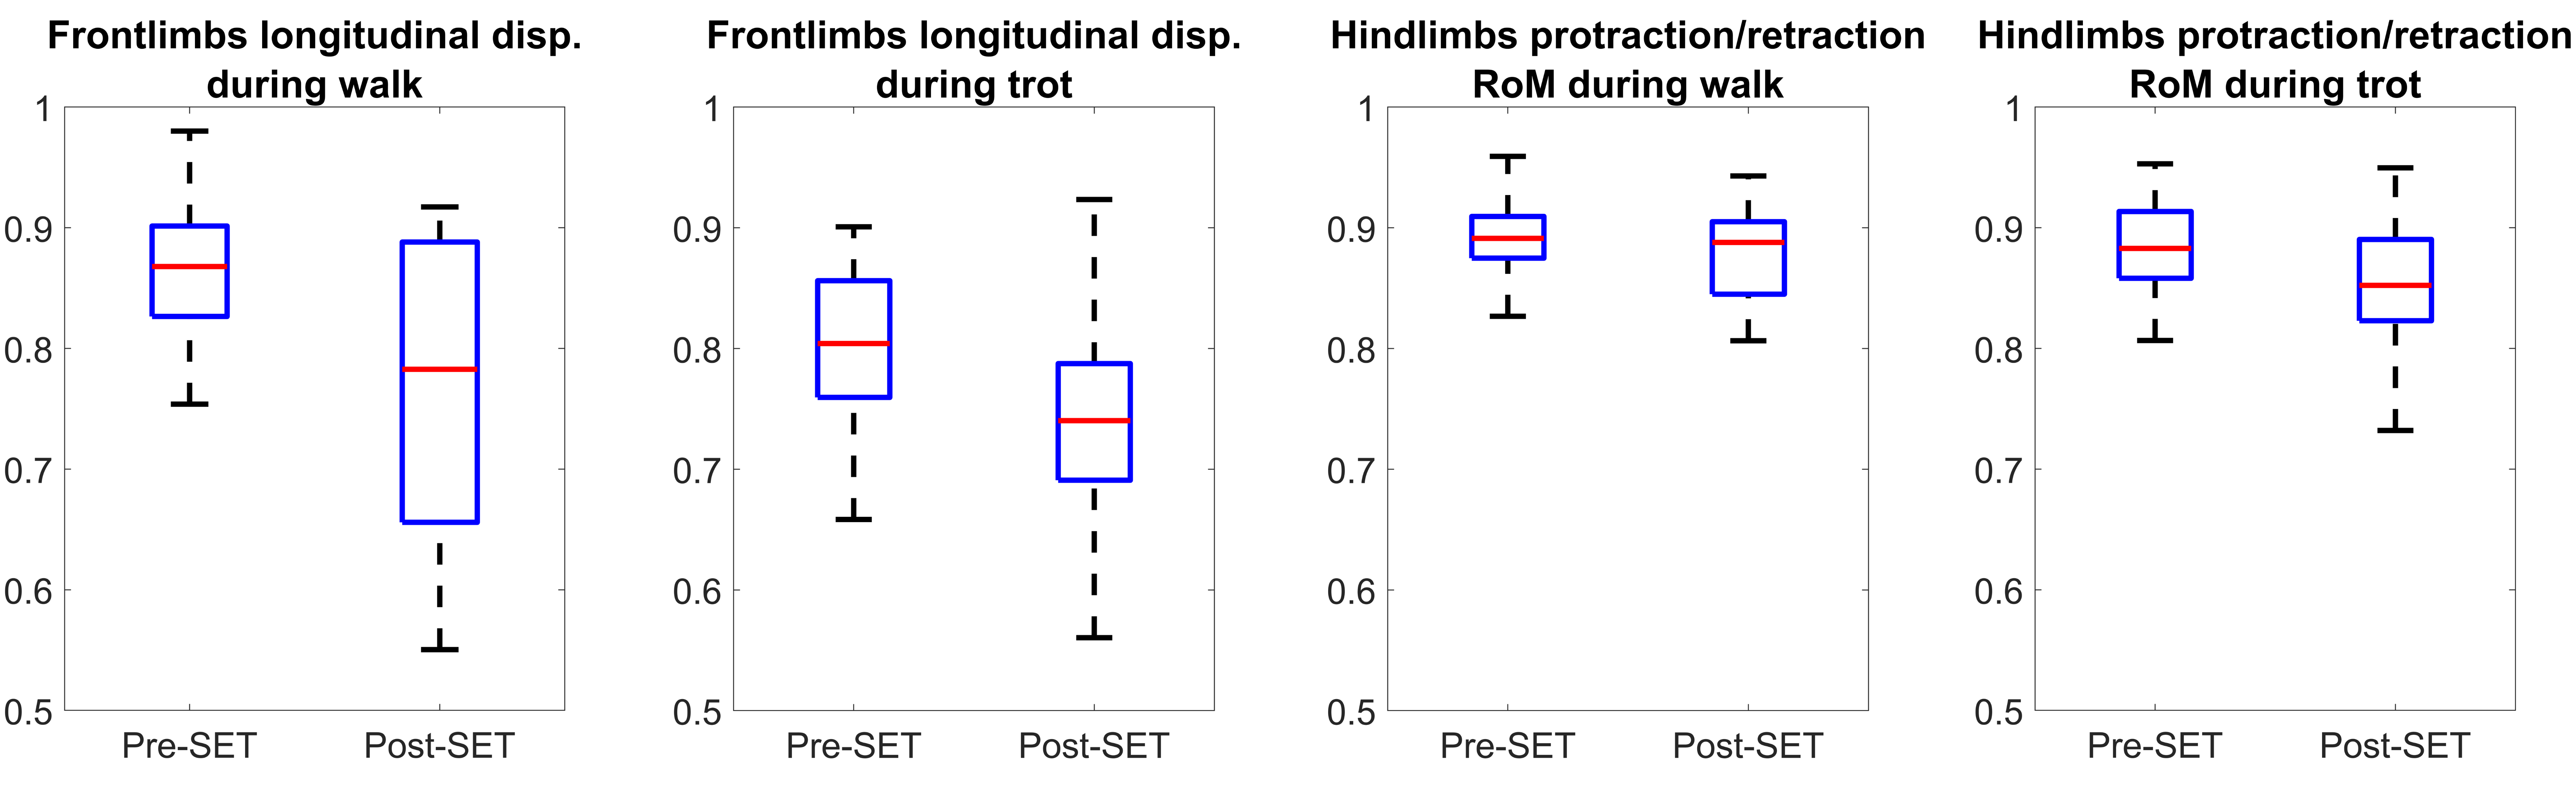
\includegraphics[width=.95\linewidth]{chapters/prepost/figures/walktrot_HQ.png}
\caption{Comparison of biomechanical features of all horses between pre-\gls{set} and post-\gls{set} during walk and trot. The vertical axes of all plots represent the range-normalized value. The box represents the interquartile range, while the red line (horizontal line within the box) shows the median value.}
\label{walktrot}
\end{figure}

\begin{figure}[htbp]
\centering

\includegraphics[width=.95\linewidth]{chapters/prepost/figures/walk_HQ.png}
\caption{Comparison of speed and stride, stance, and swing duration features of all horses between pre-\gls{set} and post-\gls{set} during walk. The vertical axes of all plots represent the range-normalized value. The box represents the interquartile range, while the red line (horizontal line within the box) shows the median value.}
\label{walk}
\end{figure}

\begin{figure}[htbp]
\centering

\includegraphics[width=.95\linewidth]{chapters/prepost/figures/trot_HQ.png}
\caption{Comparison of speed and stride, stance, and swing duration features of all horses between pre-\gls{set} and post-\gls{set} during trot. The vertical axes of all plots represent the range-normalized value. The box represents the interquartile range, while the red line (horizontal line within the box) shows the median value.}
\label{trot}
\end{figure}

\begin{figure}[!htbp]
\centering
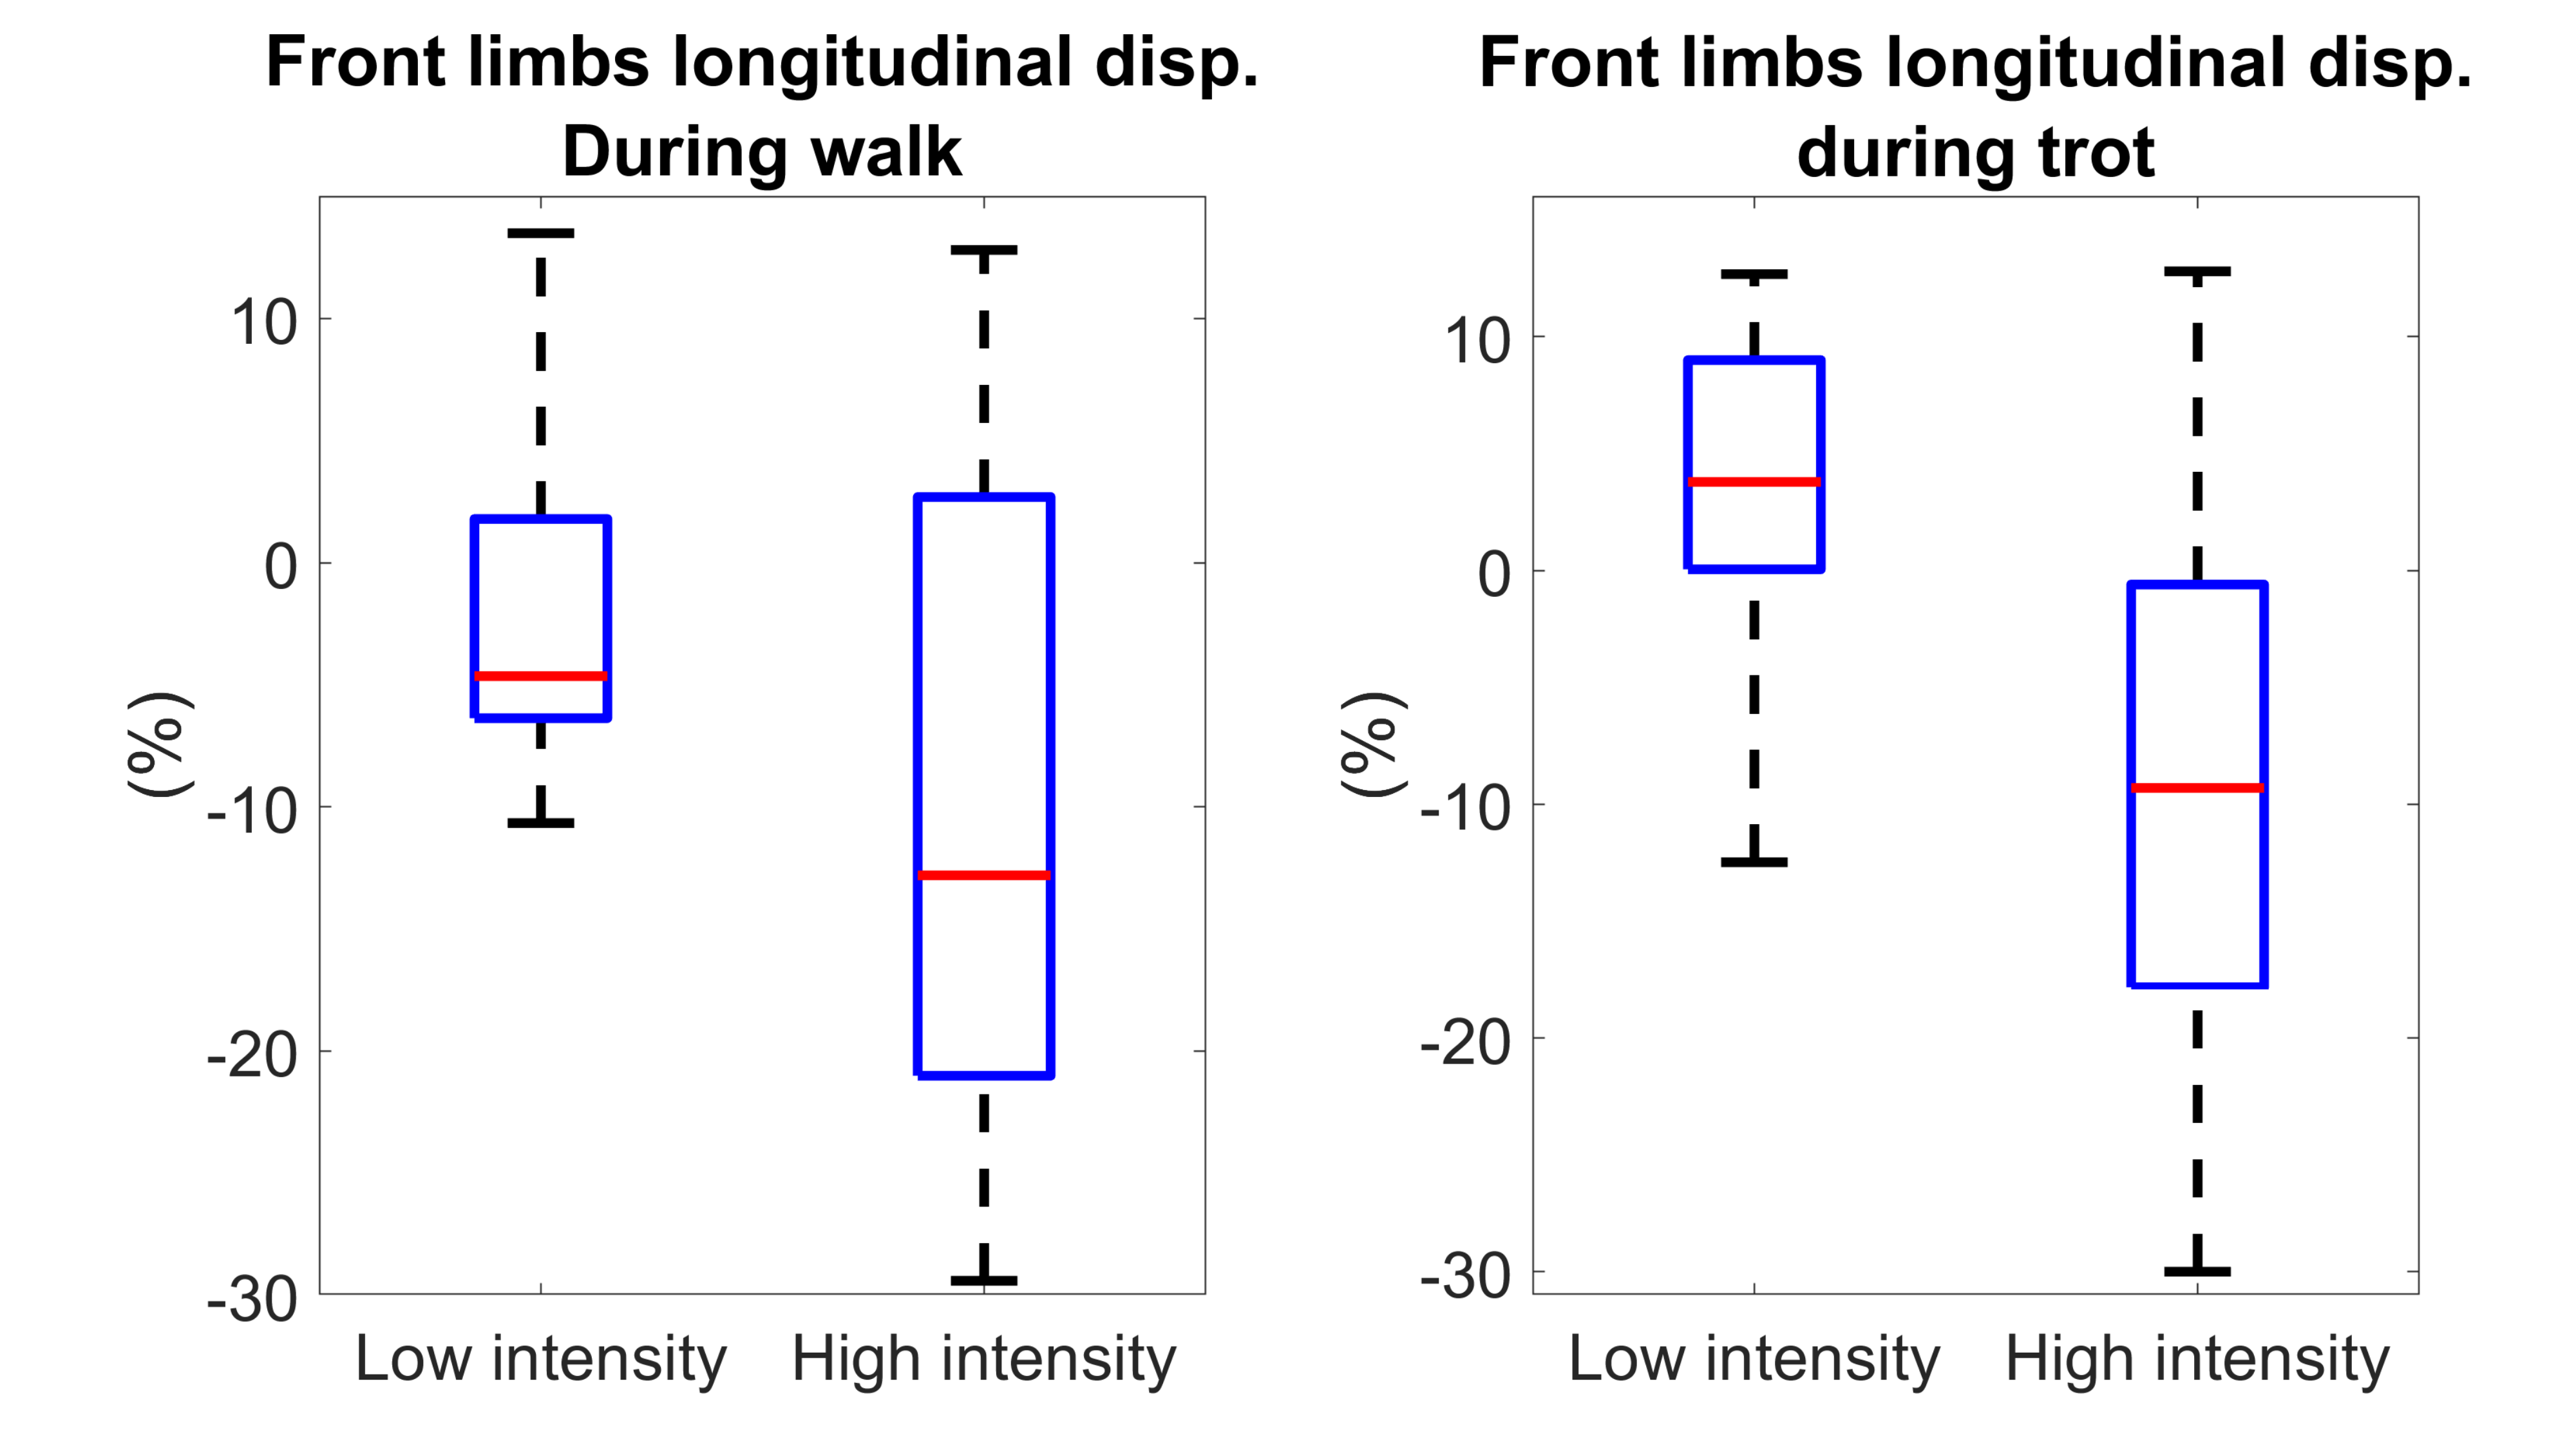
\includegraphics[scale=0.06]{chapters/prepost/figures/long_pp_HQ.png}
\caption{Comparison of biomechanical features between low and high intensity \gls{set} performers during walk and trot. The box represents the interquartile range, while the red line (horizontal line within the box) shows the median value.}
\label{prepostlong}
\end{figure}

\begin{figure}[!htbp]
\centering
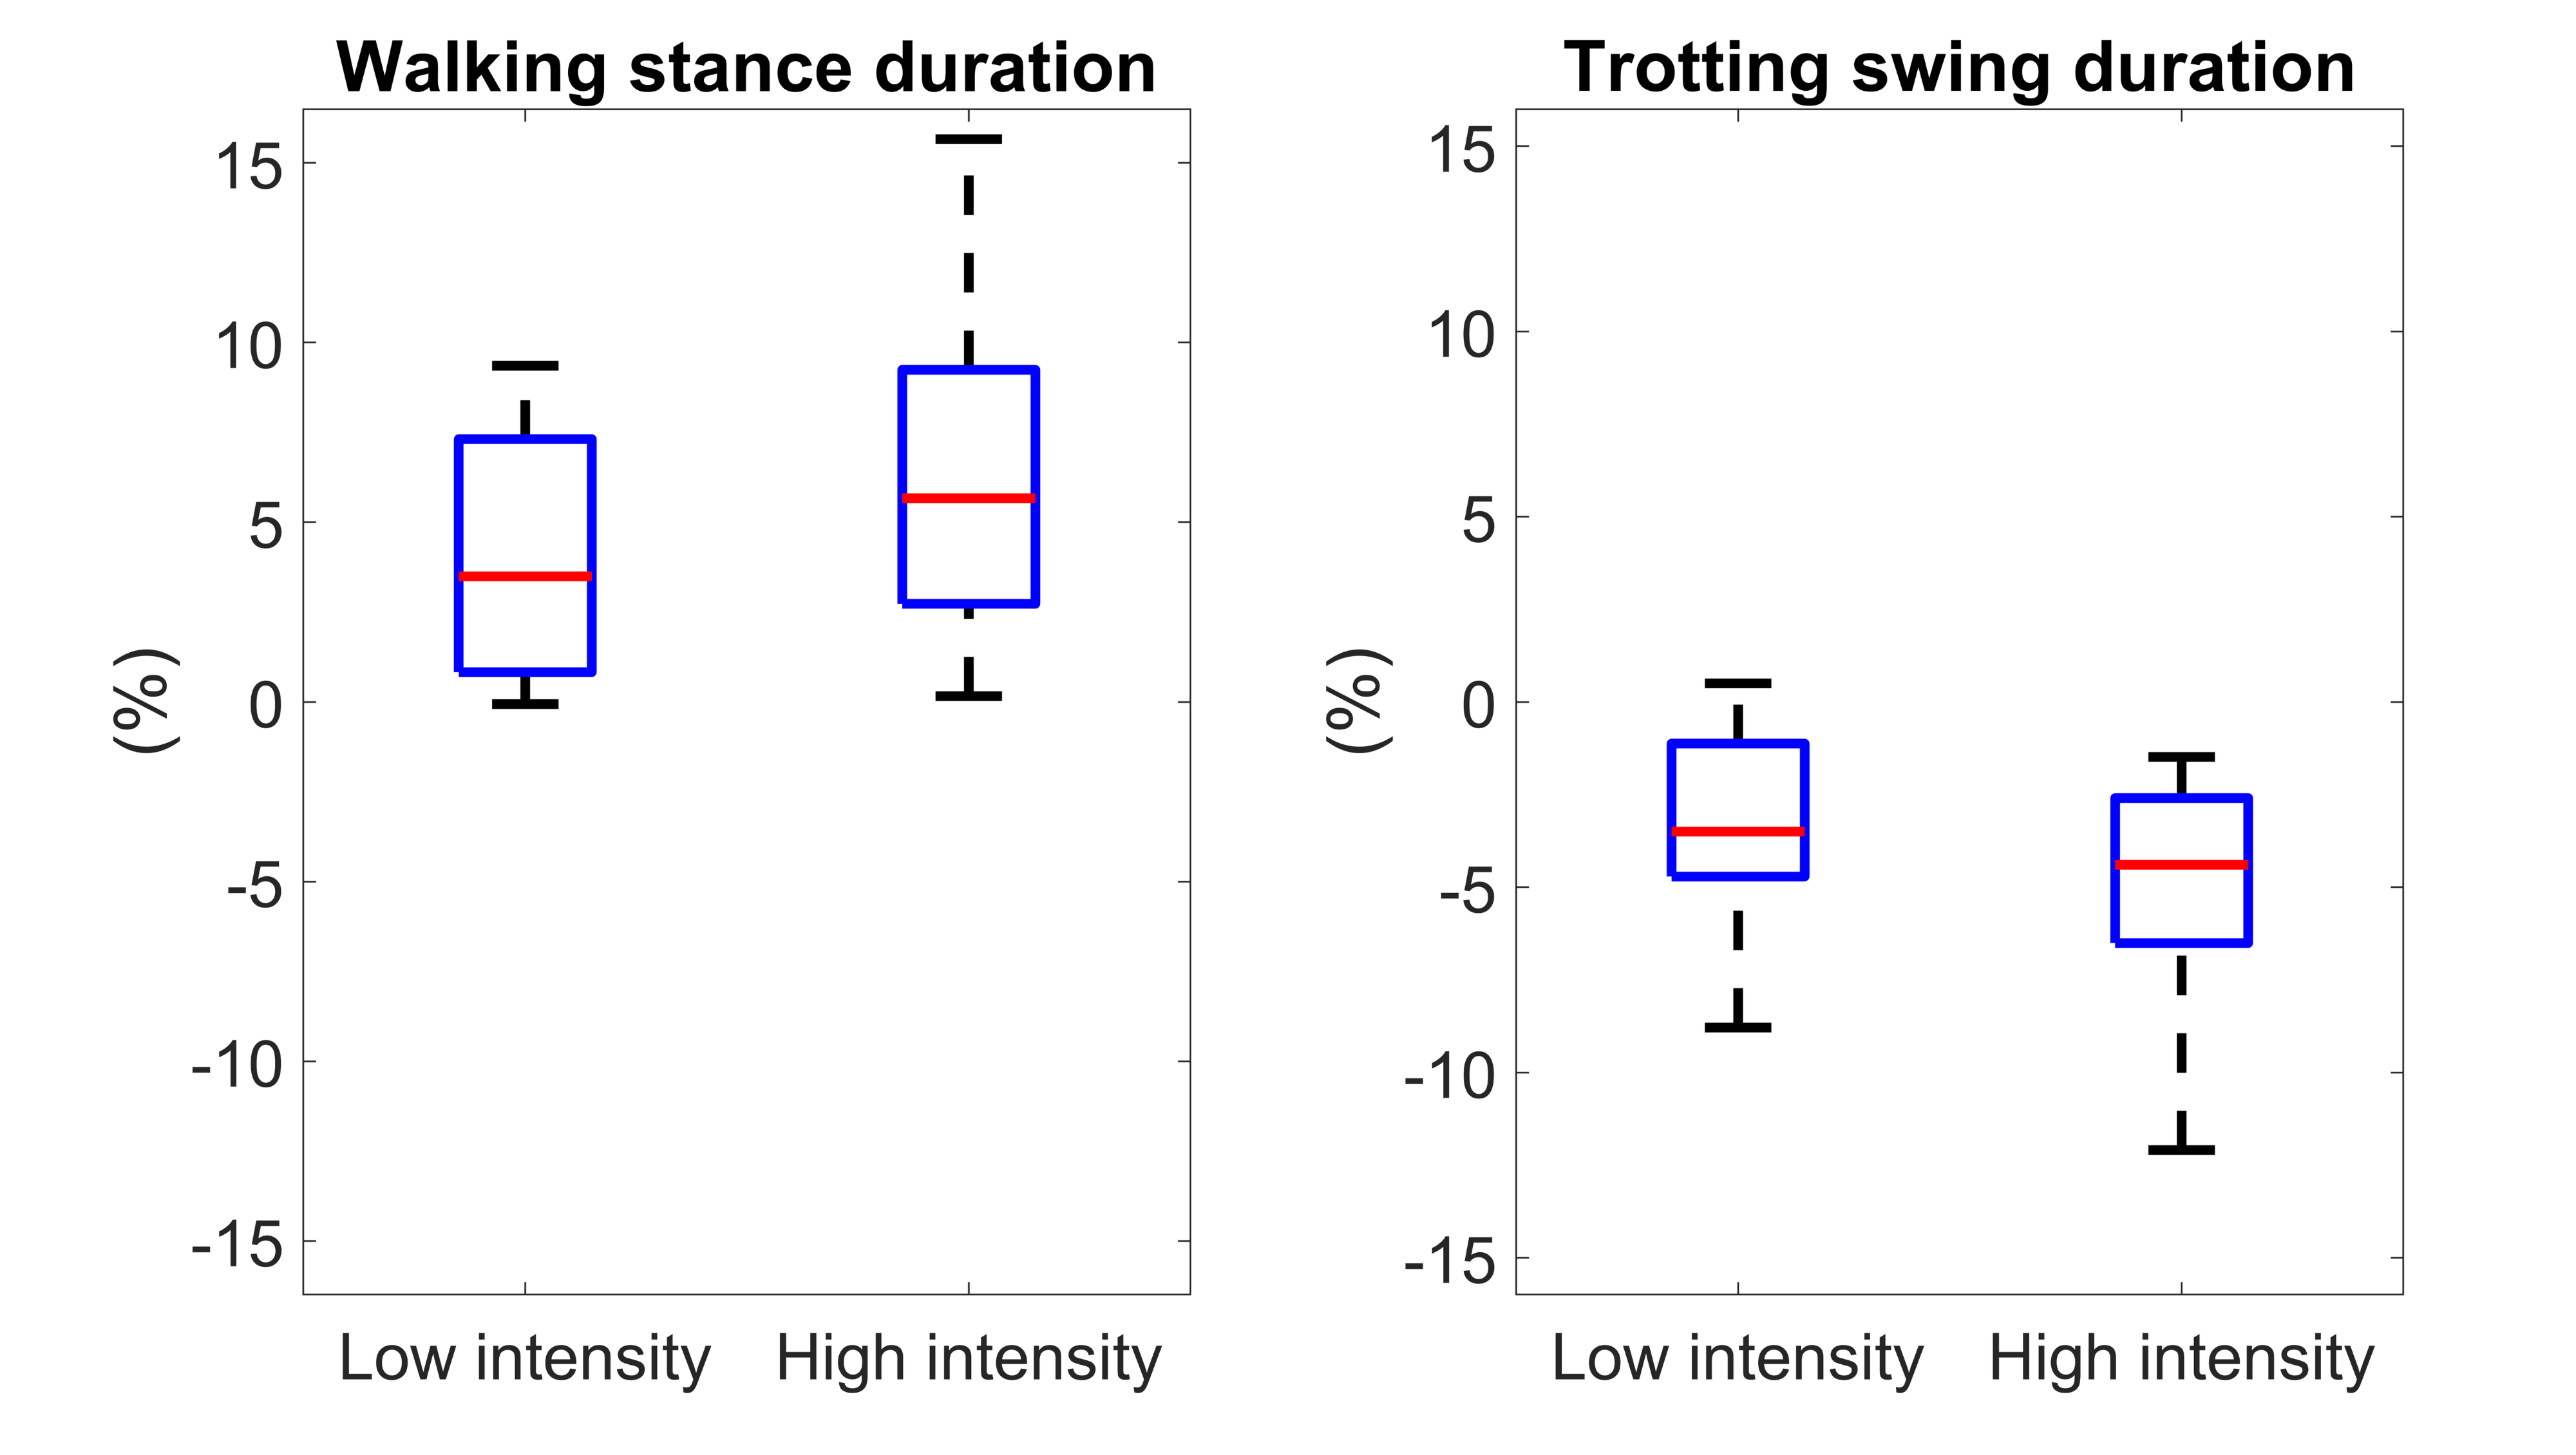
\includegraphics[scale=0.06]{chapters/prepost/figures/stride_pp_HQ.png}
\caption{Comparison of stance and swing duration between low and high intensity \gls{set} performers during walk and trot. The box represents the interquartile range, while the red line (horizontal line within the box) shows the median value.}
\label{prepoststride}
\end{figure}

\begin{figure}[!htbp]
\centering
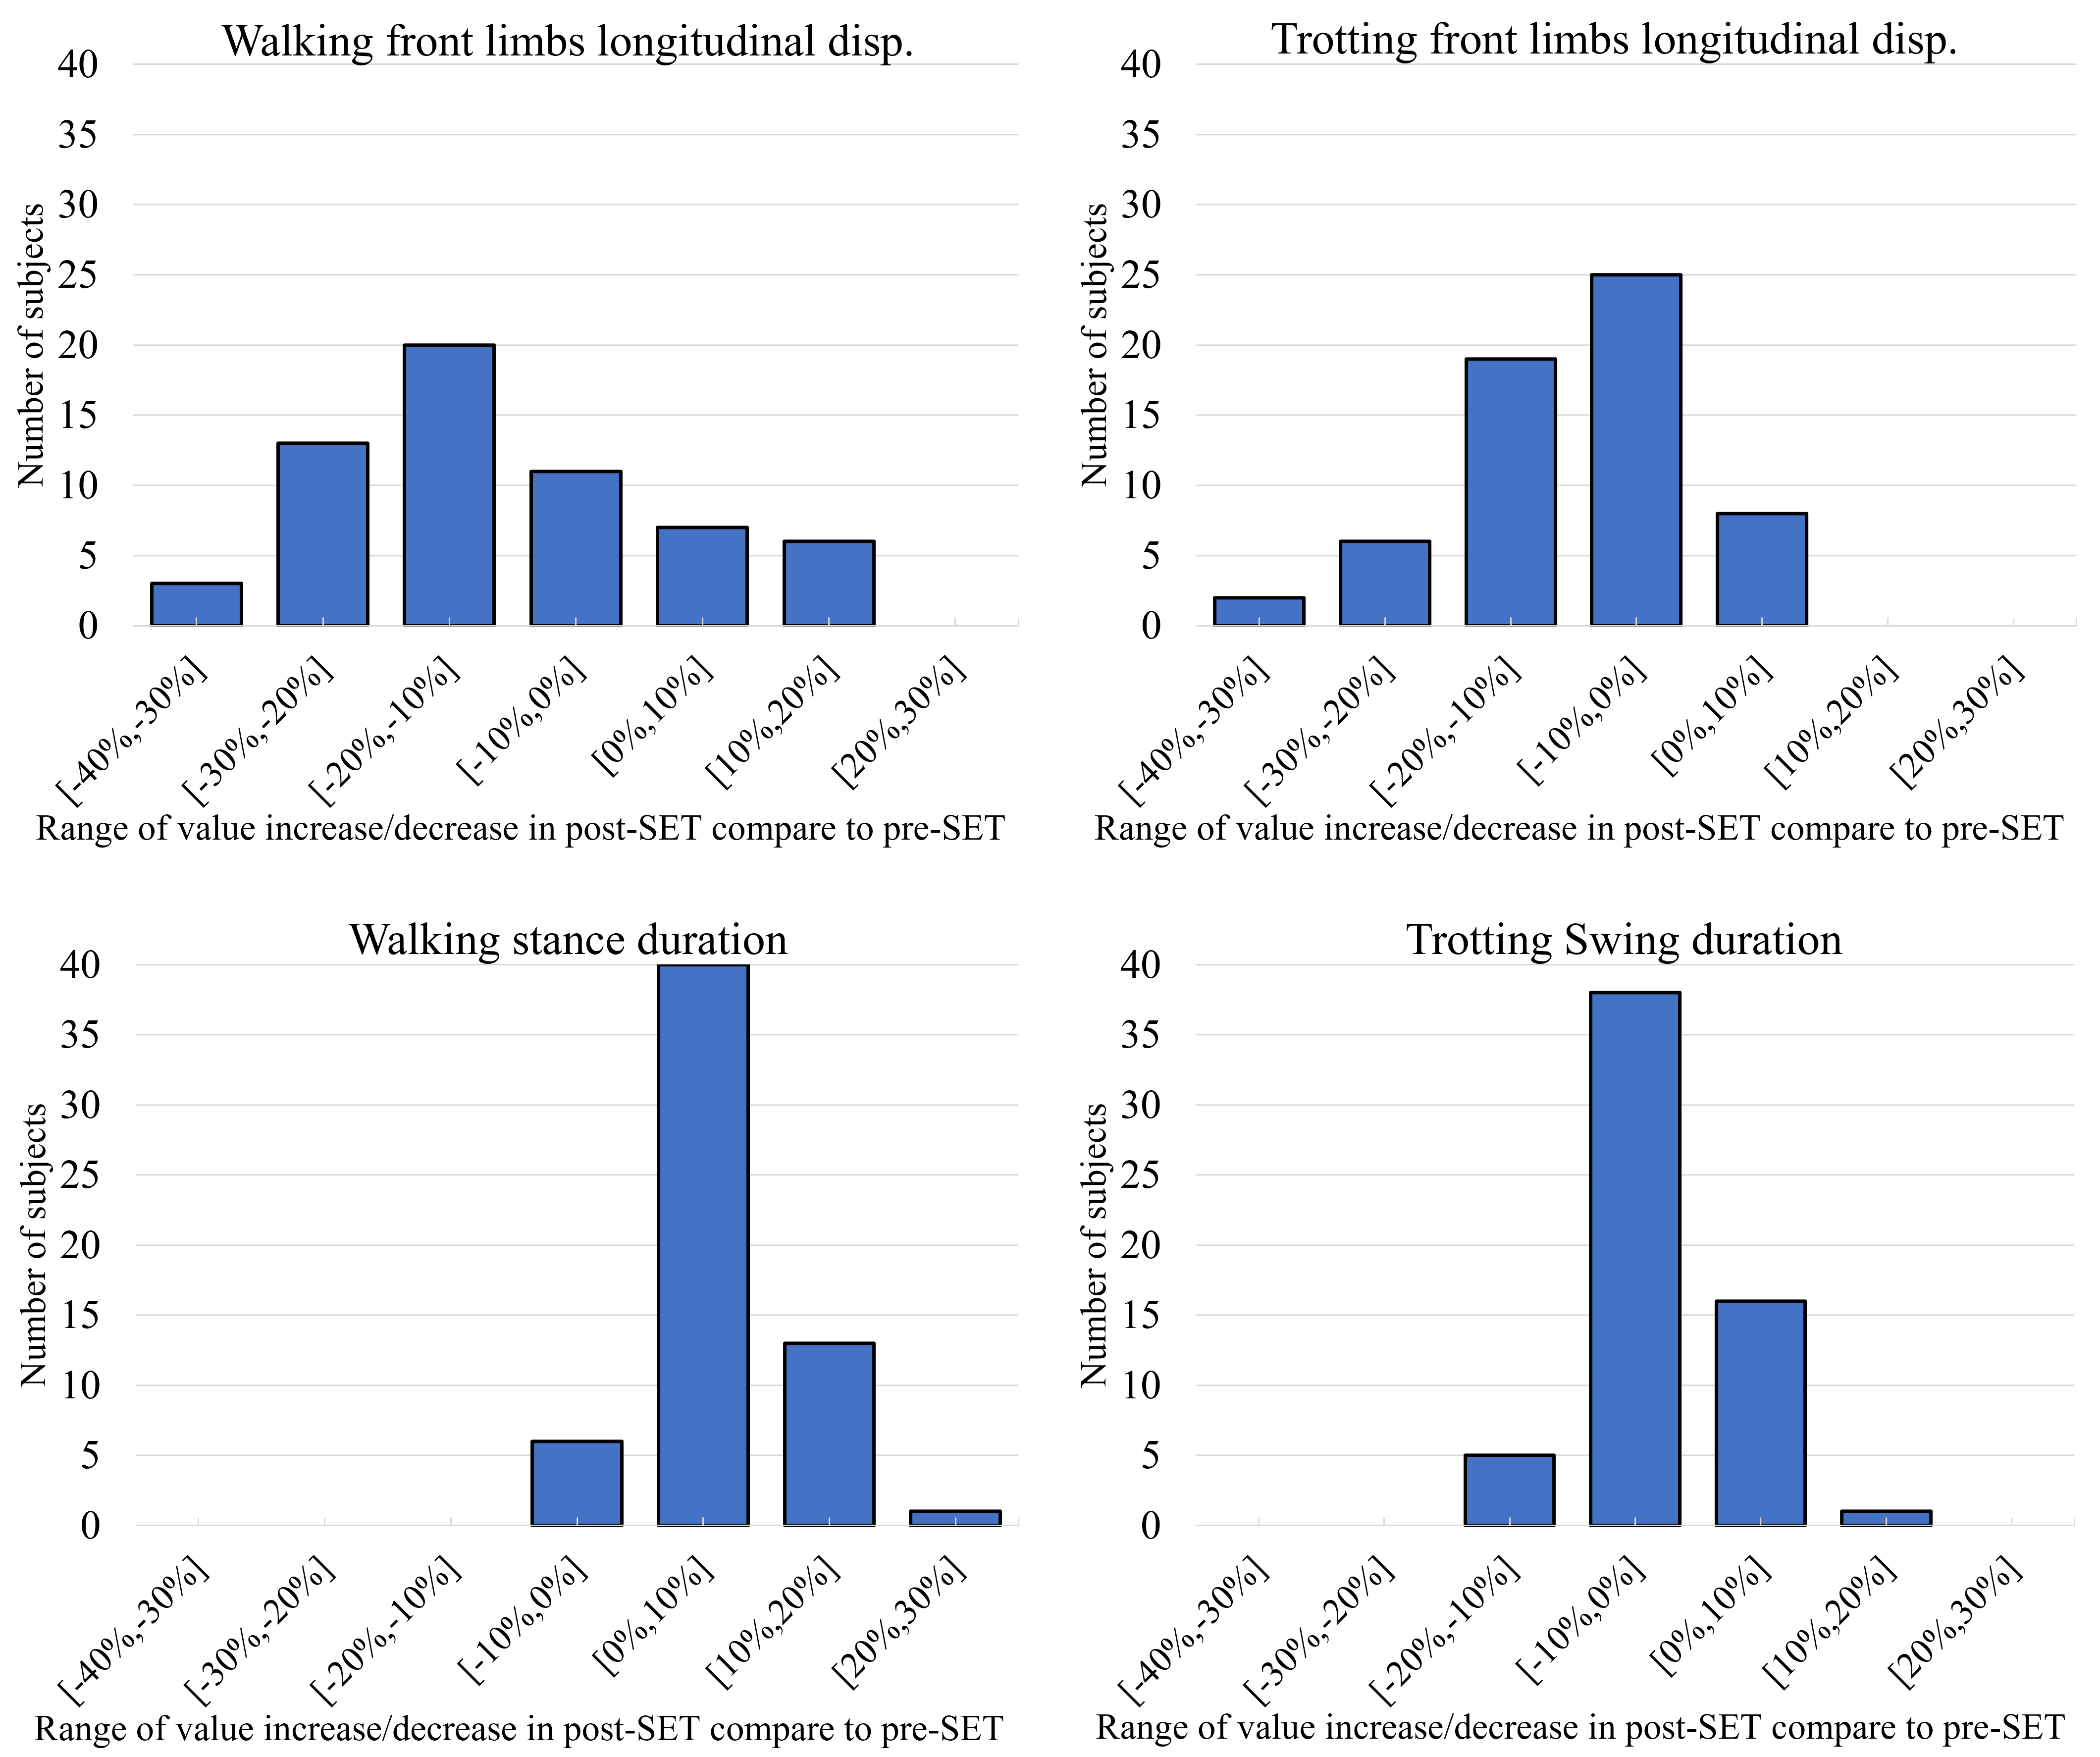
\includegraphics[width=.95\linewidth]{chapters/prepost/figures/ind_walktrot_HQ.png}
\caption{Number of horses with increased/decreased (in percentage) features values in post-\gls{set} compare to pre-\gls{set}. The vertical axis of all plots represents the range of increase (if positive) or decrease (if negative) of the specified feature value. Each bar represents the number of horses that have an increase or decrease of value within the specified range.}
\label{ind_walktrot}
\end{figure}


According to Table \ref{featuresss results}, the selected indicators by the feature selection method were mostly gait events durations features, limbs longitudinal displacement, protraction/retraction range of motion, and abduction/adduction range of motion.

Among the selected indicators, the longitudinal displacement of front limbs was presented in all subsets. For simplicity, the features from both front and hind limbs were considered features from "front limbs" and "hind limbs", respectively. None of the upper body extracted features were selected from the poll (head). The angular ranges of motions of the sacrum were selected in five of the nine subsets. The yaw angle and vertical ranges of motions were selected as important fatigue indicators for withers.

The effect of variability metrics for each subset on the model performance is presented in Table \ref{tab:variability_prepost}. Each of the four variability metrics was reported at least in one subset as the better performer in terms of accuracy. Standard deviation was chosen six times, while variance, root mean square, and coefficient of variation performed better each in one subset.

\begin{table}[!htbp] 
    \centering
      \caption{Effect of different variability metrics on the performance of the models, reported as mean ± standard deviation}% Add 'table' caption

    
    \resizebox{0.8\linewidth}{!}{% 
    \begin{tabular}{llcccc}
    
    \toprule
 
\multicolumn{1}{l}{\multirow{2}{*}{Datasets}}&\multirow{2}{*}{Subsets} & \multicolumn{4}{c}{Variability Metrics}\\ 

\cline{3-6} 

\multicolumn{1}{l}{}& & VAR^1 & CV^2 & SD^3 & RMS^4 \\ \hline

\multirow{3}{*}{\begin{tabular}[c]{@{}l@{}}Dataset 1\\ 

(High/low intensity)\end{tabular}} & Walk & 77±2\% & 82±2\% & 88±2\% & 95±2\%\\[0.4 em]

& Trot& 83±1\% & 73±1\% & 77±1\% & 77±1\% \\[0.4 em]

& Walk+Trot& 70±2\%& 72±2\%& 82±2\%& 80±2\%\\[0.4 em] 

\hline

\multirow{3}{*}{\begin{tabular}[c]{@{}l@{}}Dataset 2\\ 

(High intensity)\end{tabular}}& Walk& 82±2\% & 86±2\%& 95±2\%& 88±2\%\\[0.4 em]

& Trot& 80±4\% & 72±4\%& 86±4\%& 80±4\%\\[0.4 em]

& Walk+Trot& 80±2\%   & 72±2\%& 78±2\%& 76±2\% \\[0.4 em] 
\hline

\multirow{3}{*}{\begin{tabular}[c]{@{}l@{}}Dataset 3\\ 

(Low intensity)\end{tabular}}& Walk& 80±2\%& 80±2\%& 100±0\%& 90±2\%\\

& Trot& 73±2\%& 73±2\%& 88±2\%& 70±2\%\\[0.4 em]

& Walk+Trot& 75±3\%   & 73±3\%& 88±3\%& 83±3\%\\[0.4 em] \bottomrule

\multicolumn{6}{l}{\footnotesize{\textsuperscript{1}\textit{Variance}, \textsuperscript{2}\textit{Coefficient of variation}, \textsuperscript{3}\textit{Standard deviation}, \textsuperscript{4}\textit{Root mean square}}}\\

\end{tabular}}
\label{tab:variability_prepost}
\end{table}


The best-performing algorithm was \gls{svm} with a linear kernel and the performance results were presented in Table \ref{featuresss results}. It can be inferred from the Table that the accuracy results of classifying walking strides using the selected walking features (95\% - 100\%) were higher than classifying trot (83\% - 88\%) and Walk+Trot (80\% - 83\%) strides using their selected features. 

In the following sections, a detailed report of Table \ref{featuresss results} and the important indicators per gait and \gls{set} intensity were discussed:

%\subsection{Effect of \gls{set} intensity during walk}

The indicators of fatigue during the walk were dependent on the intensity, except stance duration, as shown in Figure \ref{prepoststride}. In \gls{set} with higher intensity, longitudinal displacement of front limbs, hind limbs protraction/retraction, withers vertical displacement, and sacrum roll angle range of motion were the important indicators, while for the indicators of the lower intensity, we identified longitudinal and mediolateral displacements and adduction/abduction of front limb, protraction/retraction of the hind limb, and withers yaw angle range of motion. Independent of the intensity, stance duration, longitudinal displacement and adduction/abduction of front limbs, and protraction/retraction of hind limbs were the most indicative parameters of fatigue. 

%\subsection{Effect of \gls{set} intensity during trot}
As depicted in Figure \ref{prepostlong}, the longitudinal displacement of front limbs was important, independent of \gls{set} intensity. However, despite the importance of mediolateral displacement of the front limbs for high-intensity \gls{set}, it was not selected as an important indicator for the low intensity \gls{set}. Instead, the adduction/abduction and retraction/protraction of the hind limb and sacrum yaw angle were important indicators of low intensity \gls{set} response. 

%\subsection{Effect of \gls{set} intensity independent of gait type}
The selected parameters as important indicators during high intensity \gls{set} were from the front limb only. However, for the low intensity \gls{set}, the roll angle of sacrum and withers were also selected. Longitudinal displacement and adduction/abduction of both front and hind limbs, and sacrum yaw angle range of motion were chosen as significant parameters if the data is analyzed independently of gait type and \gls{set} intensity.

%\subsection{Effect of gait type during higher intensity \gls{set}}
For higher intensity \gls{set}, the walking, trotting, and Walk+Trot subsets have only the longitudinal displacement of the front limbs in common. The parameters during trot and Walk+Trot were only from front limbs, while parameters extracted from front limbs, hind limbs, sacrum, and withers were important fatigue indicators during walk, in this dataset.

%\subsection{Effect of gait type during lower intensity \gls{set}}
The selected parameters for low intensity \gls{set} had the same situation as high intensity \gls{set}, there were no common indicators between walking and trotting, except the longitudinal displacement of the front limbs. However, the selected indicators in both walking and trotting included extracted parameters from the hind limb and front limb. The difference between the two gait types was on the upper body, where withers and sacrum yaw angles were selected in walking and trotting, respectively.

%\subsection{Effect of gait type independent of \gls{set} intensity}
If we do not consider the intensity of \gls{set}, the sacrum roll angle and front and hind limb protraction/retraction were important indicators during trot, while the adduction/abduction of front limbs during walk before and after \gls{set}s was significant. Front limb longitudinal displacement and hind limb protraction/retraction angle were the other indicators of training response on horses during walk, respectively. 


